% Options for packages loaded elsewhere
\PassOptionsToPackage{unicode}{hyperref}
\PassOptionsToPackage{hyphens}{url}
%
\documentclass[
]{article}
\usepackage{amsmath,amssymb}
\usepackage{lmodern}
\usepackage{iftex}
\ifPDFTeX
  \usepackage[T1]{fontenc}
  \usepackage[utf8]{inputenc}
  \usepackage{textcomp} % provide euro and other symbols
\else % if luatex or xetex
  \usepackage{unicode-math}
  \defaultfontfeatures{Scale=MatchLowercase}
  \defaultfontfeatures[\rmfamily]{Ligatures=TeX,Scale=1}
\fi
% Use upquote if available, for straight quotes in verbatim environments
\IfFileExists{upquote.sty}{\usepackage{upquote}}{}
\IfFileExists{microtype.sty}{% use microtype if available
  \usepackage[]{microtype}
  \UseMicrotypeSet[protrusion]{basicmath} % disable protrusion for tt fonts
}{}
\makeatletter
\@ifundefined{KOMAClassName}{% if non-KOMA class
  \IfFileExists{parskip.sty}{%
    \usepackage{parskip}
  }{% else
    \setlength{\parindent}{0pt}
    \setlength{\parskip}{6pt plus 2pt minus 1pt}}
}{% if KOMA class
  \KOMAoptions{parskip=half}}
\makeatother
\usepackage{xcolor}
\usepackage[margin=1in]{geometry}
\usepackage{color}
\usepackage{fancyvrb}
\newcommand{\VerbBar}{|}
\newcommand{\VERB}{\Verb[commandchars=\\\{\}]}
\DefineVerbatimEnvironment{Highlighting}{Verbatim}{commandchars=\\\{\}}
% Add ',fontsize=\small' for more characters per line
\usepackage{framed}
\definecolor{shadecolor}{RGB}{248,248,248}
\newenvironment{Shaded}{\begin{snugshade}}{\end{snugshade}}
\newcommand{\AlertTok}[1]{\textcolor[rgb]{0.94,0.16,0.16}{#1}}
\newcommand{\AnnotationTok}[1]{\textcolor[rgb]{0.56,0.35,0.01}{\textbf{\textit{#1}}}}
\newcommand{\AttributeTok}[1]{\textcolor[rgb]{0.77,0.63,0.00}{#1}}
\newcommand{\BaseNTok}[1]{\textcolor[rgb]{0.00,0.00,0.81}{#1}}
\newcommand{\BuiltInTok}[1]{#1}
\newcommand{\CharTok}[1]{\textcolor[rgb]{0.31,0.60,0.02}{#1}}
\newcommand{\CommentTok}[1]{\textcolor[rgb]{0.56,0.35,0.01}{\textit{#1}}}
\newcommand{\CommentVarTok}[1]{\textcolor[rgb]{0.56,0.35,0.01}{\textbf{\textit{#1}}}}
\newcommand{\ConstantTok}[1]{\textcolor[rgb]{0.00,0.00,0.00}{#1}}
\newcommand{\ControlFlowTok}[1]{\textcolor[rgb]{0.13,0.29,0.53}{\textbf{#1}}}
\newcommand{\DataTypeTok}[1]{\textcolor[rgb]{0.13,0.29,0.53}{#1}}
\newcommand{\DecValTok}[1]{\textcolor[rgb]{0.00,0.00,0.81}{#1}}
\newcommand{\DocumentationTok}[1]{\textcolor[rgb]{0.56,0.35,0.01}{\textbf{\textit{#1}}}}
\newcommand{\ErrorTok}[1]{\textcolor[rgb]{0.64,0.00,0.00}{\textbf{#1}}}
\newcommand{\ExtensionTok}[1]{#1}
\newcommand{\FloatTok}[1]{\textcolor[rgb]{0.00,0.00,0.81}{#1}}
\newcommand{\FunctionTok}[1]{\textcolor[rgb]{0.00,0.00,0.00}{#1}}
\newcommand{\ImportTok}[1]{#1}
\newcommand{\InformationTok}[1]{\textcolor[rgb]{0.56,0.35,0.01}{\textbf{\textit{#1}}}}
\newcommand{\KeywordTok}[1]{\textcolor[rgb]{0.13,0.29,0.53}{\textbf{#1}}}
\newcommand{\NormalTok}[1]{#1}
\newcommand{\OperatorTok}[1]{\textcolor[rgb]{0.81,0.36,0.00}{\textbf{#1}}}
\newcommand{\OtherTok}[1]{\textcolor[rgb]{0.56,0.35,0.01}{#1}}
\newcommand{\PreprocessorTok}[1]{\textcolor[rgb]{0.56,0.35,0.01}{\textit{#1}}}
\newcommand{\RegionMarkerTok}[1]{#1}
\newcommand{\SpecialCharTok}[1]{\textcolor[rgb]{0.00,0.00,0.00}{#1}}
\newcommand{\SpecialStringTok}[1]{\textcolor[rgb]{0.31,0.60,0.02}{#1}}
\newcommand{\StringTok}[1]{\textcolor[rgb]{0.31,0.60,0.02}{#1}}
\newcommand{\VariableTok}[1]{\textcolor[rgb]{0.00,0.00,0.00}{#1}}
\newcommand{\VerbatimStringTok}[1]{\textcolor[rgb]{0.31,0.60,0.02}{#1}}
\newcommand{\WarningTok}[1]{\textcolor[rgb]{0.56,0.35,0.01}{\textbf{\textit{#1}}}}
\usepackage{graphicx}
\makeatletter
\def\maxwidth{\ifdim\Gin@nat@width>\linewidth\linewidth\else\Gin@nat@width\fi}
\def\maxheight{\ifdim\Gin@nat@height>\textheight\textheight\else\Gin@nat@height\fi}
\makeatother
% Scale images if necessary, so that they will not overflow the page
% margins by default, and it is still possible to overwrite the defaults
% using explicit options in \includegraphics[width, height, ...]{}
\setkeys{Gin}{width=\maxwidth,height=\maxheight,keepaspectratio}
% Set default figure placement to htbp
\makeatletter
\def\fps@figure{htbp}
\makeatother
\setlength{\emergencystretch}{3em} % prevent overfull lines
\providecommand{\tightlist}{%
  \setlength{\itemsep}{0pt}\setlength{\parskip}{0pt}}
\setcounter{secnumdepth}{-\maxdimen} % remove section numbering
\ifLuaTeX
  \usepackage{selnolig}  % disable illegal ligatures
\fi
\IfFileExists{bookmark.sty}{\usepackage{bookmark}}{\usepackage{hyperref}}
\IfFileExists{xurl.sty}{\usepackage{xurl}}{} % add URL line breaks if available
\urlstyle{same} % disable monospaced font for URLs
\hypersetup{
  pdftitle={HUDM6026 Homework\_07},
  pdfauthor={Chenguang Pan},
  hidelinks,
  pdfcreator={LaTeX via pandoc}}

\title{HUDM6026 Homework\_07}
\author{Chenguang Pan}
\date{Mar 17, 2023}

\begin{document}
\maketitle

\hypertarget{q1}{%
\subsection{Q1:}\label{q1}}

\emph{Do some research on the two-sample Kolmogorov-Smirnov (K-S) test
for equality of distributions. Describe the null and alternative
hypotheses and discuss how the test statistic is computed}

\textbf{MY SOLUTION:}

\textbf{{[}Part of my answer for this question refered to ChatGPT's
responses, crosschecked with Wikipedia{]}}

\hypertarget{two-sample-k-s-tests-concept}{%
\subsubsection{1.1 Two sample K-S test's
concept}\label{two-sample-k-s-tests-concept}}

The two-sample Kolmogorov-Smirnov(K-S) test is a nonparametric test used
to test whether two datasets are from the same population. K-S test
works by comparing the cumulative distribution functions (CDF) of the
two datasets.

The null hypothesis is that two datasets are drawn from the same
population or that they have the same underlying probability
distributions. The alternative hypothesis is that they are not from the
same population or that they do not have the same underlying probability
distributions. That is,
\[H_0: F_1(x)=F_2(x) \quad\text{ v.s. }\quad H_1: F_1(x)\neq F_2(x)\],
where \(F_1(x)\) and \(F_2(x)\) are the distributions of two sets of
random variables \(X_1\) and \(X_2\).

\hypertarget{how-to-compute-the-two-sample-k-s-test}{%
\subsubsection{1.2 How to compute the two-sample K-S
test}\label{how-to-compute-the-two-sample-k-s-test}}

The K-S test compares the largest vertical distance between the two
empirical cumulative distribution functions(ECDF). This is also called
the Kolmogorov-Smirnov statistic (D). The test statistic is defined as:
\[D=max|F_1(x)-F_2(x)|\], where \(F_1(x)\) and \(F_2(x)\) are the ECDF
of two datasets being compared.\\
The maximum distance (i.e., the \(D\)) between the two CDFs is then
compared to a critical value
\[c(\alpha)\cdot\sqrt{\frac{m+n}{m\cdot n}}\], where
\(c(\alpha)= \sqrt{-0.5ln(0.5\alpha)}\), depending on the sample size
and significance level chosen.

If the test statistic is greater than the critical value, the null
hypothesis is rejected, indicating that the two sets of data are not
drawn from the same population.

\hypertarget{q2}{%
\subsection{Q2:}\label{q2}}

\emph{Install package MatchIt and load it. Then call data(lalonde).
Examine the help on lalonde and describe the meaning of the treat and
re78 variables.}

\textbf{MY SOLUTION:}

\begin{Shaded}
\begin{Highlighting}[]
\SpecialCharTok{\textgreater{}} \FunctionTok{install.packages}\NormalTok{(}\StringTok{"MatchIt"}\NormalTok{)}
\end{Highlighting}
\end{Shaded}

\begin{Shaded}
\begin{Highlighting}[]
\SpecialCharTok{\textgreater{}} \CommentTok{\# extract the basic information of the given dataset}
\ErrorTok{\textgreater{}} \FunctionTok{library}\NormalTok{(MatchIt)}
\SpecialCharTok{\textgreater{}} \FunctionTok{data}\NormalTok{(lalonde)}
\SpecialCharTok{\textgreater{}} \FunctionTok{head}\NormalTok{(lalonde)}
\NormalTok{     treat age educ   race married nodegree re74 re75       re78}
\NormalTok{NSW1     }\DecValTok{1}  \DecValTok{37}   \DecValTok{11}\NormalTok{  black       }\DecValTok{1}        \DecValTok{1}    \DecValTok{0}    \DecValTok{0}  \FloatTok{9930.0460}
\NormalTok{NSW2     }\DecValTok{1}  \DecValTok{22}    \DecValTok{9}\NormalTok{ hispan       }\DecValTok{0}        \DecValTok{1}    \DecValTok{0}    \DecValTok{0}  \FloatTok{3595.8940}
\NormalTok{NSW3     }\DecValTok{1}  \DecValTok{30}   \DecValTok{12}\NormalTok{  black       }\DecValTok{0}        \DecValTok{0}    \DecValTok{0}    \DecValTok{0} \FloatTok{24909.4500}
\NormalTok{NSW4     }\DecValTok{1}  \DecValTok{27}   \DecValTok{11}\NormalTok{  black       }\DecValTok{0}        \DecValTok{1}    \DecValTok{0}    \DecValTok{0}  \FloatTok{7506.1460}
\NormalTok{NSW5     }\DecValTok{1}  \DecValTok{33}    \DecValTok{8}\NormalTok{  black       }\DecValTok{0}        \DecValTok{1}    \DecValTok{0}    \DecValTok{0}   \FloatTok{289.7899}
\NormalTok{NSW6     }\DecValTok{1}  \DecValTok{22}    \DecValTok{9}\NormalTok{  black       }\DecValTok{0}        \DecValTok{1}    \DecValTok{0}    \DecValTok{0}  \FloatTok{4056.4940}
\SpecialCharTok{\textgreater{}} \FunctionTok{dim}\NormalTok{(lalonde)}
\NormalTok{[}\DecValTok{1}\NormalTok{] }\DecValTok{614}   \DecValTok{9}
\end{Highlighting}
\end{Shaded}

The help file shows that \texttt{lalonde} has one treated group from NSW
with the size of 185 and one comparison group from PSID with the size of
429. The variable \texttt{treat} is the treatment assignment(1= treated,
0=control). The \texttt{re78} is income in 1978, in US dollars.

\hypertarget{q3}{%
\subsection{Q3:}\label{q3}}

\emph{Run the two-sample K-S test to test if participant income in 1978
is identically distributed across treatment group assignment or
not\ldots{}}

\textbf{MY SOLUTION:}

\begin{Shaded}
\begin{Highlighting}[]
\SpecialCharTok{\textgreater{}} \CommentTok{\# subset the treatment and control groups}
\ErrorTok{\textgreater{}}\NormalTok{ x }\OtherTok{\textless{}{-}}\NormalTok{ lalonde}\SpecialCharTok{$}\NormalTok{re78[lalonde}\SpecialCharTok{$}\NormalTok{treat }\SpecialCharTok{==}\DecValTok{1}\NormalTok{]}
\SpecialCharTok{\textgreater{}}\NormalTok{ y }\OtherTok{\textless{}{-}}\NormalTok{ lalonde}\SpecialCharTok{$}\NormalTok{re78[lalonde}\SpecialCharTok{$}\NormalTok{treat }\SpecialCharTok{==}\DecValTok{0}\NormalTok{]}
\SpecialCharTok{\textgreater{}} 
\ErrorTok{\textgreater{}} \CommentTok{\# run the two sample k{-}s test}
\ErrorTok{\textgreater{}} \FunctionTok{ks.test}\NormalTok{(x, y)}

\NormalTok{    Asymptotic two}\SpecialCharTok{{-}}\NormalTok{sample Kolmogorov}\SpecialCharTok{{-}}\NormalTok{Smirnov test}

\NormalTok{data}\SpecialCharTok{:}\NormalTok{  x and y}
\NormalTok{D }\OtherTok{=} \FloatTok{0.098608}\NormalTok{, p}\SpecialCharTok{{-}}\NormalTok{value }\OtherTok{=} \FloatTok{0.1619}
\NormalTok{alternative hypothesis}\SpecialCharTok{:}\NormalTok{ two}\SpecialCharTok{{-}}\NormalTok{sided}
\end{Highlighting}
\end{Shaded}

The test statistic \(D\) is .0986. Since the p-value is .162 and it is
greater than the significant level .05, we fail to reject the null
hypothesis. That is, there is no statistically significant difference
between the treatment and comparison groups.

\hypertarget{q4}{%
\subsection{Q4:}\label{q4}}

\emph{Create a function that takes two arguments, x and y, each a vector
of values, and outputs the value of the two-sample K-S statistic D}

\textbf{MY SOLUTION:}

There is a function \texttt{ecdf()} built in R. I plan to use it
directly and won't write the \texttt{ecdf} function from the scratch.

\begin{Shaded}
\begin{Highlighting}[]
\SpecialCharTok{\textgreater{}}\NormalTok{ ks\_d }\OtherTok{\textless{}{-}} \ControlFlowTok{function}\NormalTok{(x, y)\{}
\SpecialCharTok{+}   \CommentTok{\# get the maximize vertical distance between the two ecdfs}
\SpecialCharTok{+}\NormalTok{   d }\OtherTok{\textless{}{-}} \FunctionTok{max}\NormalTok{(}\FunctionTok{abs}\NormalTok{(}\FunctionTok{ecdf}\NormalTok{(x)(x)}\SpecialCharTok{{-}}\FunctionTok{ecdf}\NormalTok{(y)(x)))}
\SpecialCharTok{+}   \FunctionTok{return}\NormalTok{(d)}
\SpecialCharTok{+}\NormalTok{ \}}
\end{Highlighting}
\end{Shaded}

\hypertarget{q5}{%
\subsection{Q5:}\label{q5}}

\emph{Run an approximate permutation test with B = 1000 permutation
replications to determine the estimated ASL for testing the null
hypothesis that participant incomes are identically distributed across
treatment arms. Use a = 0.05}

\textbf{MY SOLUTION:}\\
The sample sizes for treatment and control groups are 185 and 429.

\begin{Shaded}
\begin{Highlighting}[]
\SpecialCharTok{\textgreater{}} \FunctionTok{data}\NormalTok{(lalonde)}
\SpecialCharTok{\textgreater{}} \FunctionTok{set.seed}\NormalTok{(}\DecValTok{666}\NormalTok{)}
\SpecialCharTok{\textgreater{}} \CommentTok{\# subset the treatment and control group}
\ErrorTok{\textgreater{}}\NormalTok{ treat\_group }\OtherTok{\textless{}{-}}\NormalTok{ lalonde}\SpecialCharTok{$}\NormalTok{re78[lalonde}\SpecialCharTok{$}\NormalTok{treat }\SpecialCharTok{==}\DecValTok{1}\NormalTok{]}
\SpecialCharTok{\textgreater{}}\NormalTok{ control\_group }\OtherTok{\textless{}{-}}\NormalTok{ lalonde}\SpecialCharTok{$}\NormalTok{re78[lalonde}\SpecialCharTok{$}\NormalTok{treat }\SpecialCharTok{==}\DecValTok{0}\NormalTok{]}
\SpecialCharTok{\textgreater{}} \CommentTok{\# get the observed the K{-}S test\textquotesingle{}s D}
\ErrorTok{\textgreater{}}\NormalTok{ d\_observed }\OtherTok{\textless{}{-}} \FunctionTok{ks\_d}\NormalTok{(treat\_group, control\_group)}
\SpecialCharTok{\textgreater{}} \CommentTok{\# get the sample sizes of treatment and control groups}
\ErrorTok{\textgreater{}}\NormalTok{ size\_treat }\OtherTok{\textless{}{-}} \FunctionTok{length}\NormalTok{(treat\_group); size\_control }\OtherTok{\textless{}{-}} \FunctionTok{length}\NormalTok{(control\_group)}
\SpecialCharTok{\textgreater{}} \CommentTok{\# define the repeating times}
\ErrorTok{\textgreater{}}\NormalTok{ B }\OtherTok{\textless{}{-}} \DecValTok{1000}
\SpecialCharTok{\textgreater{}} \CommentTok{\# create a empty array to load the test statistic D from different permutations}
\ErrorTok{\textgreater{}}\NormalTok{ ks\_ds }\OtherTok{\textless{}{-}} \FunctionTok{rep}\NormalTok{(}\ConstantTok{NA}\NormalTok{,B)}
\SpecialCharTok{\textgreater{}} \CommentTok{\# creat a variable to count how many times the re{-}sampling Ds is greater than the }
\ErrorTok{\textgreater{}} \CommentTok{\# observed one.}
\ErrorTok{\textgreater{}}\NormalTok{ d\_bigger }\OtherTok{\textless{}{-}} \DecValTok{0}
\SpecialCharTok{\textgreater{}} 
\ErrorTok{\textgreater{}} \CommentTok{\# randomly sample data from combined dataset in the sizes of 185 and 429}
\ErrorTok{\textgreater{}} \ControlFlowTok{for}\NormalTok{ (i }\ControlFlowTok{in} \DecValTok{1}\SpecialCharTok{:}\NormalTok{B) \{}
\SpecialCharTok{+}   \CommentTok{\# randomly sample data from the whole re78 data in the size of 185+429}
\SpecialCharTok{+}\NormalTok{   dat }\OtherTok{\textless{}{-}} \FunctionTok{sample}\NormalTok{(lalonde}\SpecialCharTok{$}\NormalTok{re78)}
\SpecialCharTok{+}   \CommentTok{\# split the random sample into 185 and 429 sample sizes}
\SpecialCharTok{+}\NormalTok{   x }\OtherTok{\textless{}{-}}\NormalTok{ dat[}\DecValTok{1}\SpecialCharTok{:}\NormalTok{ size\_treat]}
\SpecialCharTok{+}\NormalTok{   y }\OtherTok{\textless{}{-}}\NormalTok{ dat[(size\_treat}\SpecialCharTok{+}\DecValTok{1}\NormalTok{)}\SpecialCharTok{:}\NormalTok{ (size\_treat}\SpecialCharTok{+}\NormalTok{size\_control)]}
\SpecialCharTok{+}   \CommentTok{\# plug the x and y into the D function above}
\SpecialCharTok{+}\NormalTok{   d\_temp }\OtherTok{\textless{}{-}} \FunctionTok{ks\_d}\NormalTok{(x,y)}
\SpecialCharTok{+}   \CommentTok{\# write the d\_temp to the ks\_ds}
\SpecialCharTok{+}\NormalTok{   ks\_ds[i] }\OtherTok{\textless{}{-}}\NormalTok{ d\_temp}
\SpecialCharTok{+}   \CommentTok{\# compare the d\_temp with the observed KS test\textquotesingle{}s D}
\SpecialCharTok{+}   \ControlFlowTok{if}\NormalTok{ (d\_temp }\SpecialCharTok{\textgreater{}=}\NormalTok{ d\_observed)\{}
\SpecialCharTok{+}\NormalTok{     d\_bigger }\OtherTok{\textless{}{-}}\NormalTok{ d\_bigger }\SpecialCharTok{+} \DecValTok{1}
\SpecialCharTok{+}\NormalTok{   \}}
\SpecialCharTok{+}\NormalTok{ \}}
\SpecialCharTok{\textgreater{}} \CommentTok{\# get the p value}
\ErrorTok{\textgreater{}}\NormalTok{ p\_value }\OtherTok{\textless{}{-}} \FunctionTok{round}\NormalTok{(d\_bigger}\SpecialCharTok{/}\NormalTok{B,}\DecValTok{3}\NormalTok{)}
\SpecialCharTok{\textgreater{}}\NormalTok{ p\_value}
\NormalTok{[}\DecValTok{1}\NormalTok{] }\FloatTok{0.116}
\SpecialCharTok{\textgreater{}} \FunctionTok{print}\NormalTok{(}\FunctionTok{paste0}\NormalTok{(}\StringTok{"The Ds from permuated data are "}\NormalTok{, }
\SpecialCharTok{+}\NormalTok{              d\_bigger, }
\SpecialCharTok{+}              \StringTok{" times greater than the observed D "}\NormalTok{,}
\SpecialCharTok{+}              \FunctionTok{round}\NormalTok{(d\_observed,}\DecValTok{3}\NormalTok{),}\StringTok{"."}\NormalTok{))}
\NormalTok{[}\DecValTok{1}\NormalTok{] }\StringTok{"The Ds from permuated data are 116 times greater than the observed D 0.099."}
\SpecialCharTok{\textgreater{}} \FunctionTok{print}\NormalTok{(}\FunctionTok{paste0}\NormalTok{(}\StringTok{"The P value is "}\NormalTok{, }
\SpecialCharTok{+}\NormalTok{              p\_value, }\StringTok{"."}\NormalTok{))}
\NormalTok{[}\DecValTok{1}\NormalTok{] }\StringTok{"The P value is 0.116."}
\end{Highlighting}
\end{Shaded}

The result shows that the re-sampling-based p value (.116) is greater
than .05. We fail to reject the null hypothesis. This calculated p value
is close to p value .162 obtained from theoretical null distribution in
Question 3.

\hypertarget{q6}{%
\subsection{Q6:}\label{q6}}

\emph{Plot a histogram of the permutation distribution created by
applying the K-S statistic to the B = 1000 permutation replications.}

\textbf{MY SOLUTION:}

\begin{Shaded}
\begin{Highlighting}[]
\SpecialCharTok{\textgreater{}} \FunctionTok{hist}\NormalTok{(ks\_ds, }\AttributeTok{breaks =}\DecValTok{100}\NormalTok{, }\AttributeTok{xlim=}\FunctionTok{c}\NormalTok{(}\DecValTok{0}\NormalTok{,}\FloatTok{0.17}\NormalTok{), }
\SpecialCharTok{+}      \AttributeTok{main=}\StringTok{"Figure 1. A histogram of the re{-}sampling{-}based test statistics"}\NormalTok{,}
\SpecialCharTok{+}      \AttributeTok{xlab=}\StringTok{"Null Distribution of Test Statistic"}\NormalTok{, }\AttributeTok{col=}\DecValTok{7}\NormalTok{)}
\end{Highlighting}
\end{Shaded}

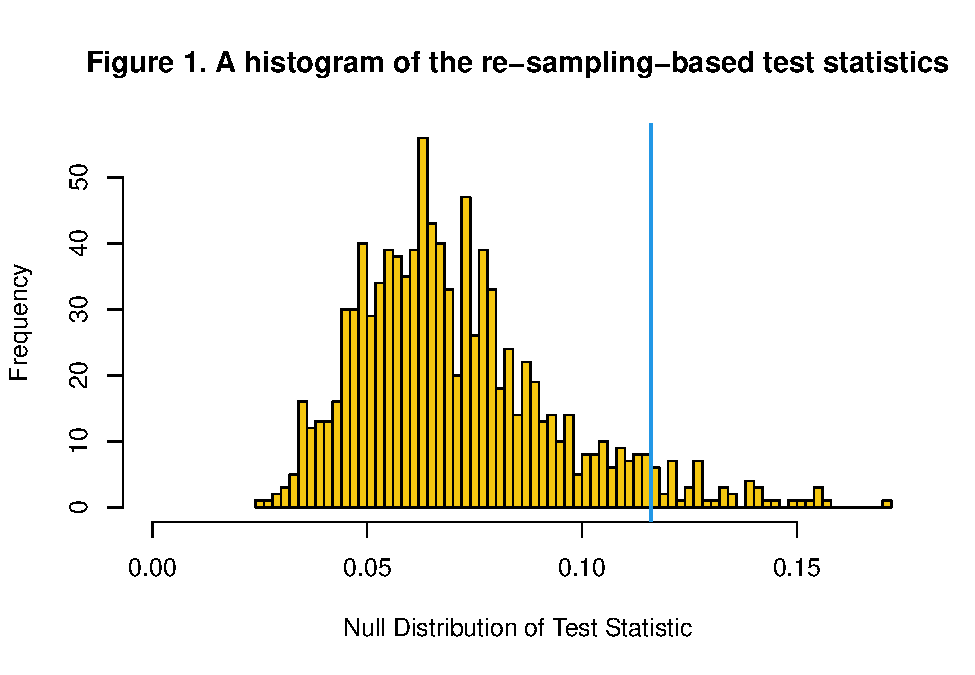
\includegraphics{Homework_07_Pan_files/figure-latex/unnamed-chunk-6-1.pdf}

\hypertarget{reference}{%
\subsection{Reference}\label{reference}}

Keller, B.(2023). \emph{HUDM 6026 Computational Statistics: 07
Permutation Test}{[}Lecture notes{]}.

In Wikipedia.(2023). \emph{Kolmogorov--Smirnov test.}
\url{https://en.wikipedia.org/wiki/Kolmogorov\%E2\%80\%93Smirnov_test}

Hastie, T., Tibshirani, R., \& Friedman, J. (2009). \emph{An
introduction to statistical learning.}

Rizzo, M. L. (2019). \emph{Statistical computing with R.} Chapman and
Hall/CRC.

\end{document}
